
%------------------------------------------------

\newpage

\section{$\chi^{2}$ distribution}
\label{exer:chisquare_distr}

\subsection{Generate $\chi^{2}$ distribution}

\begin{enumerate}
	\item Generate $10^{5}$ sets of $n$ standard normal variables $\chi$, and populate the histogram with $X^{2} = \sum_{i = 1}^{n}{\chi^{2}}$.
	\item Repeat 1. for $n = \{ 1, 2, 3, 5, 10, 20 \}$.
	\item Plot the histograms and overlap them with the theoretical $\chi^{2}$ distribution with the corresponding number of degrees of freedom, properly scaled to the number of generated values.
\end{enumerate}

(Figure~\ref{fig:chisquare_distr})

\begin{figure}
	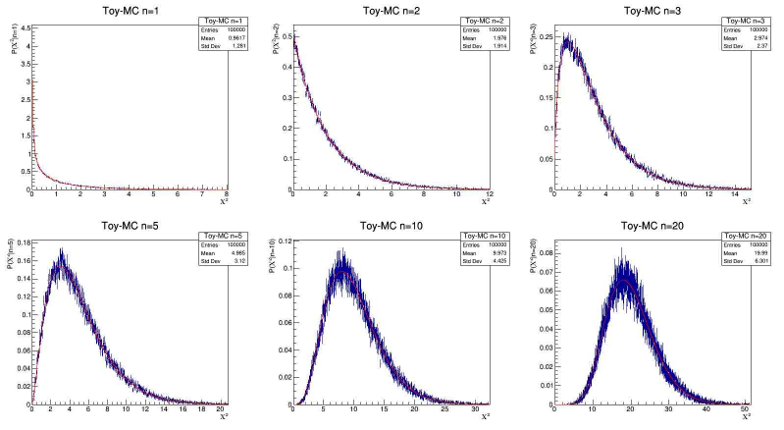
\includegraphics{exercise/chisquare_distr.png}
	\caption[$\chi^{2}$ distribution.][6pt]{$\chi^{2}$ distribution.}
	\label{fig:chisquare_distr}
\end{figure}

($\hookleftarrow$ \ref{subsec:chisquare_distr})
